\section{Excel}
Zum berechnen des Problems am Computer haben wir Excel verwendet. Wer das git repository hat, kann sich die Excel file angucken, jedoch habe ich keine Möglichkeit gefunden diese in
${\displaystyle \mathrm {L\!\!^{{}_{A}}\!\!\!\!\!\;\;T\!_{\displaystyle E}\!X}}$ 
so einzubinden, dass man es herunterladen kann.\\
Die Tabelle zu dem Problem:\\\\
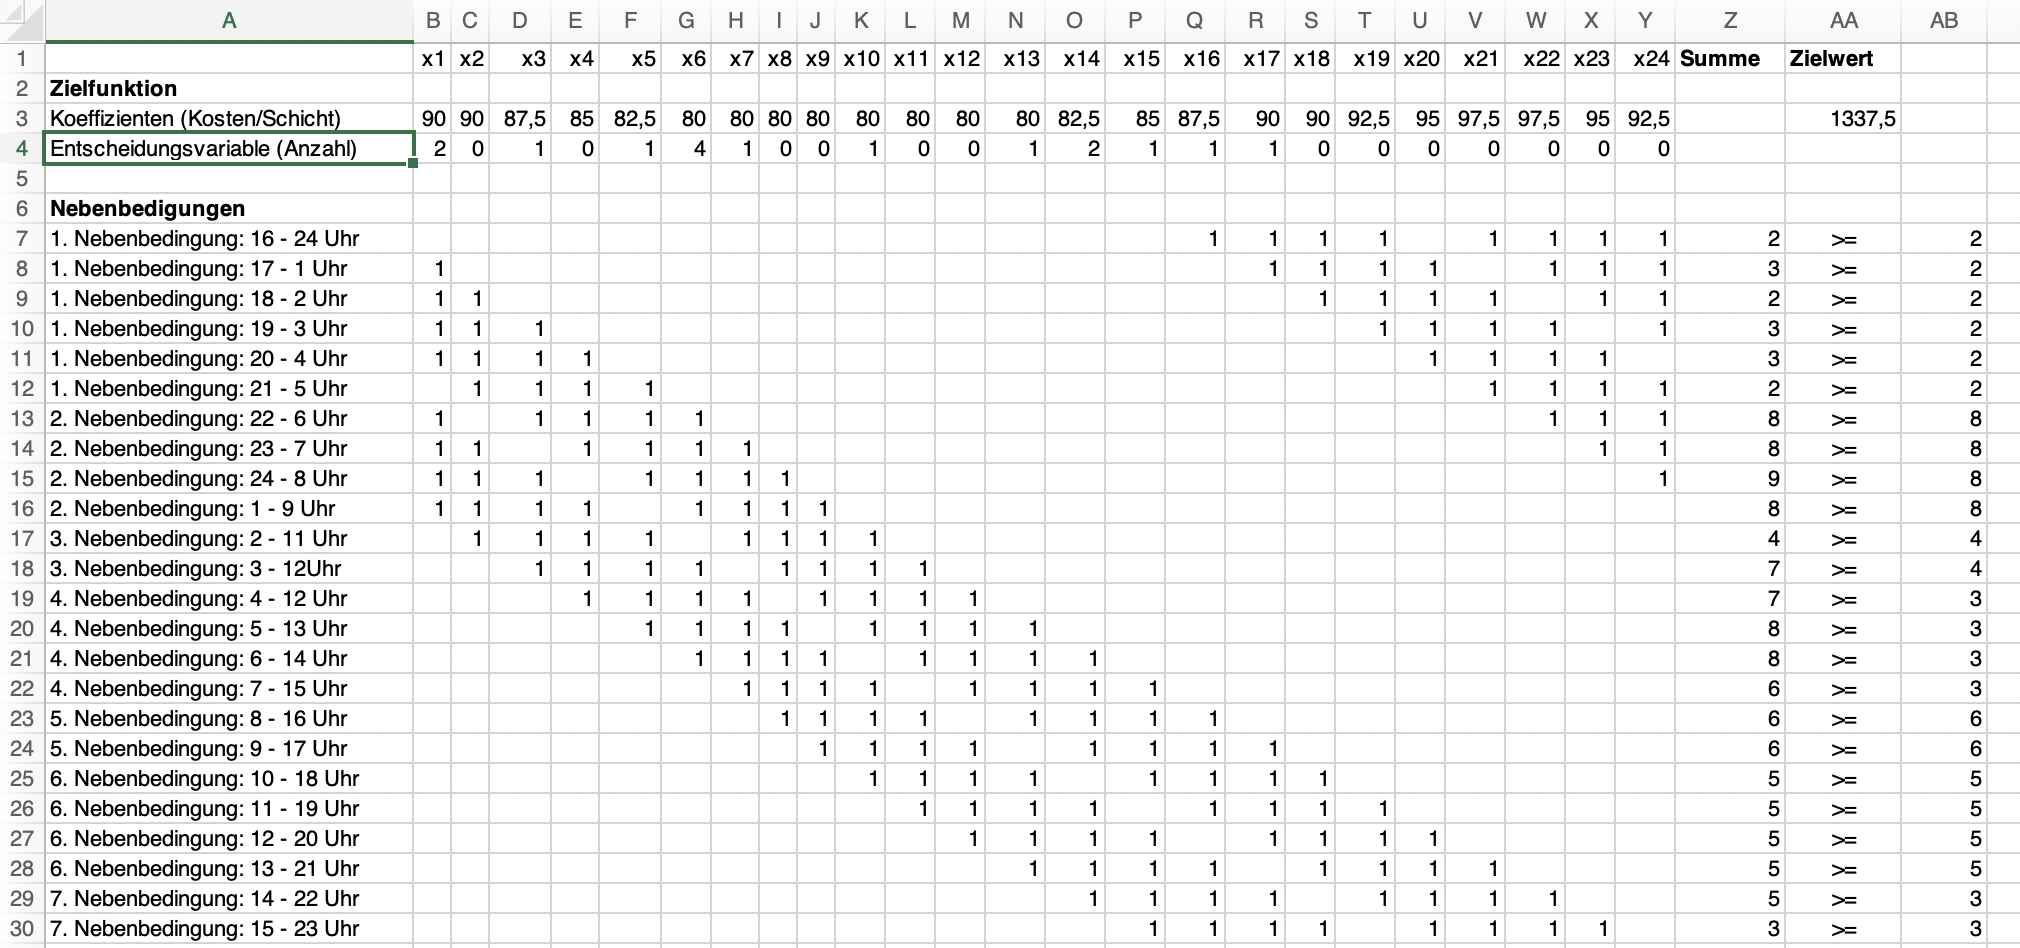
\includegraphics[width=17cm,left]{images/SimplexTabelle.png}\\
Der erste Antwortbericht:\\
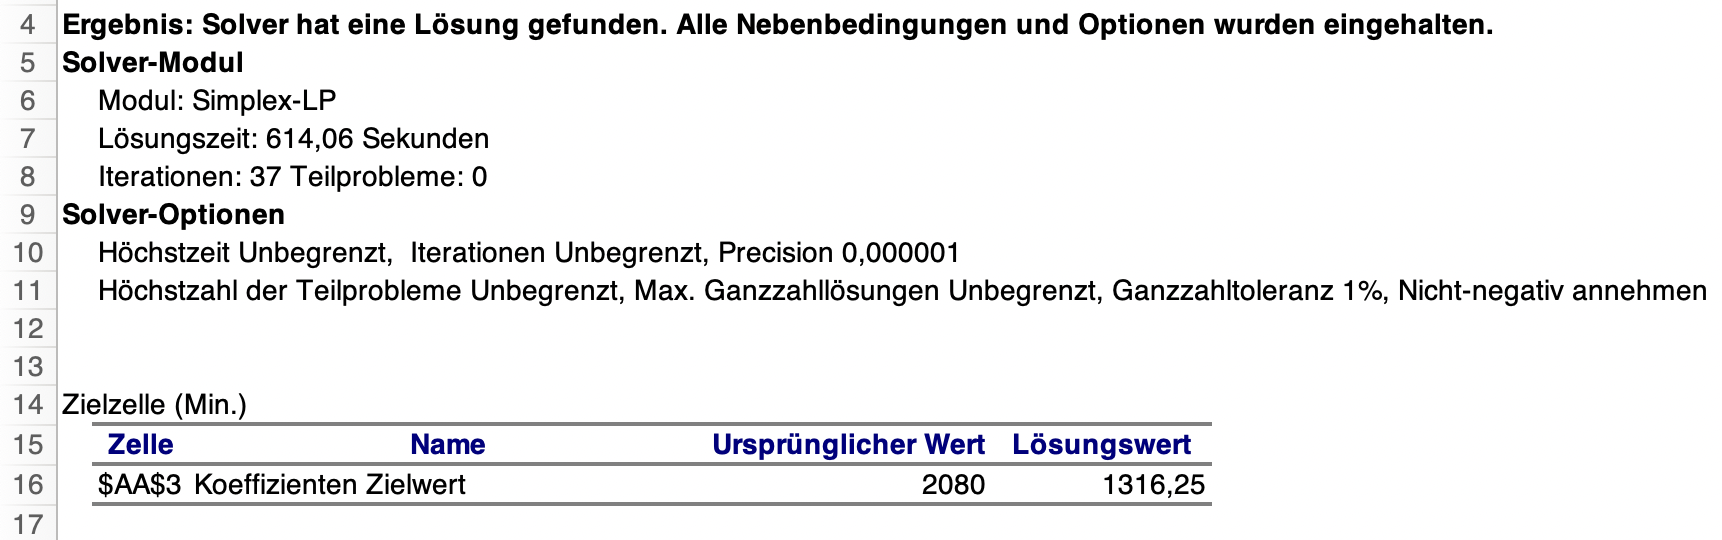
\includegraphics[width=17cm,left]{images/Antwortbericht11.png}
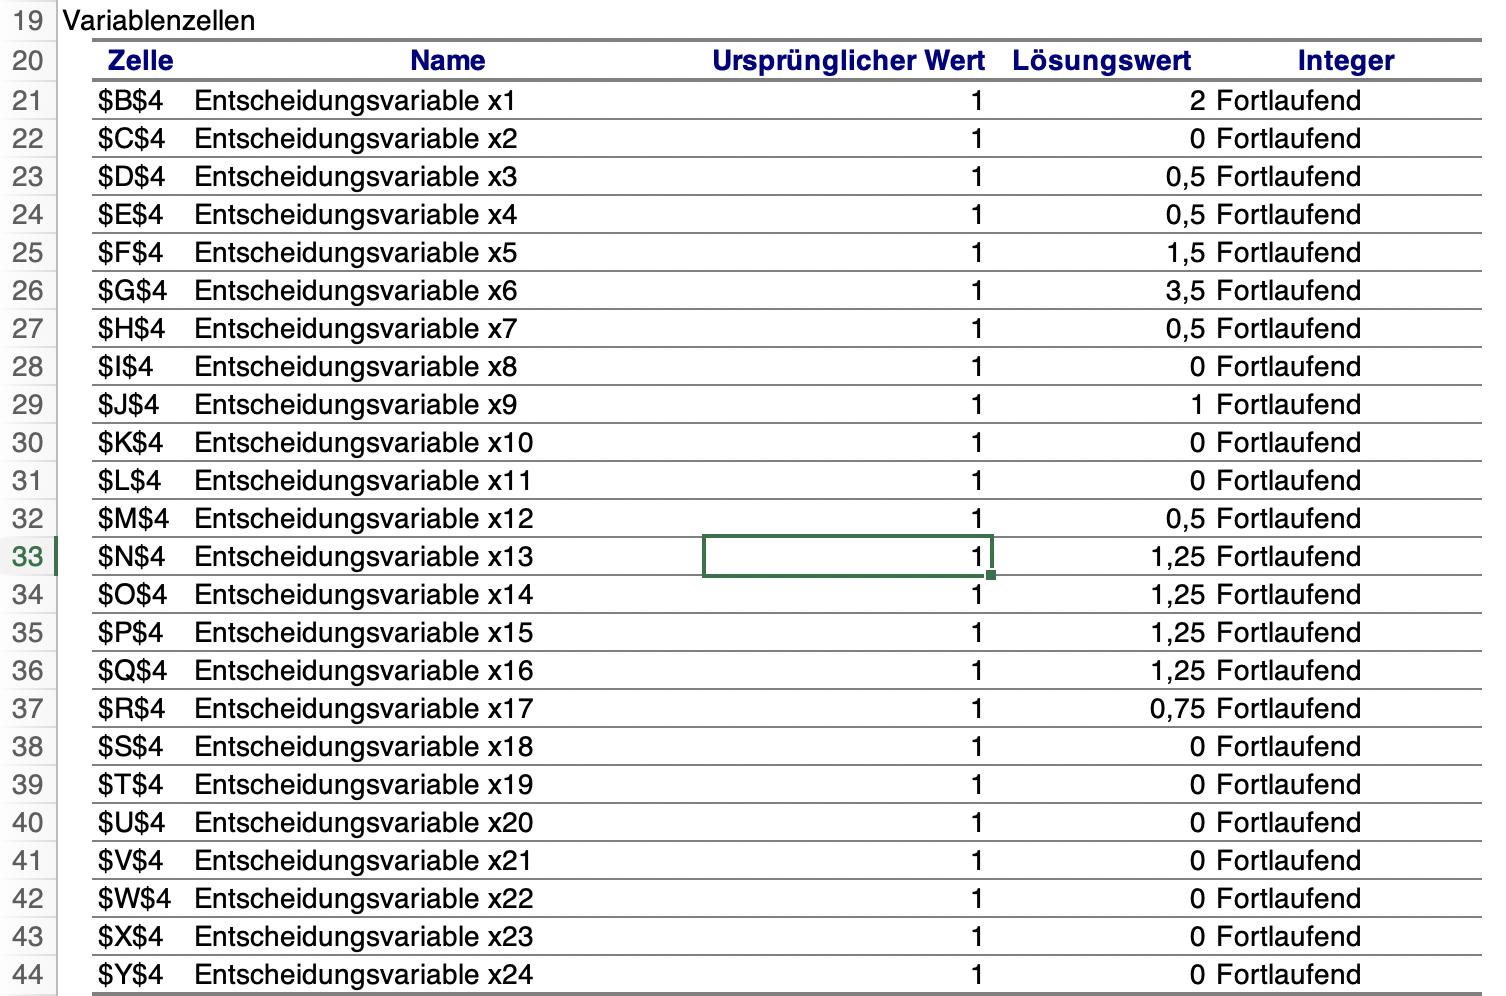
\includegraphics[width=17cm,left]{images/Antwortbericht12.png}
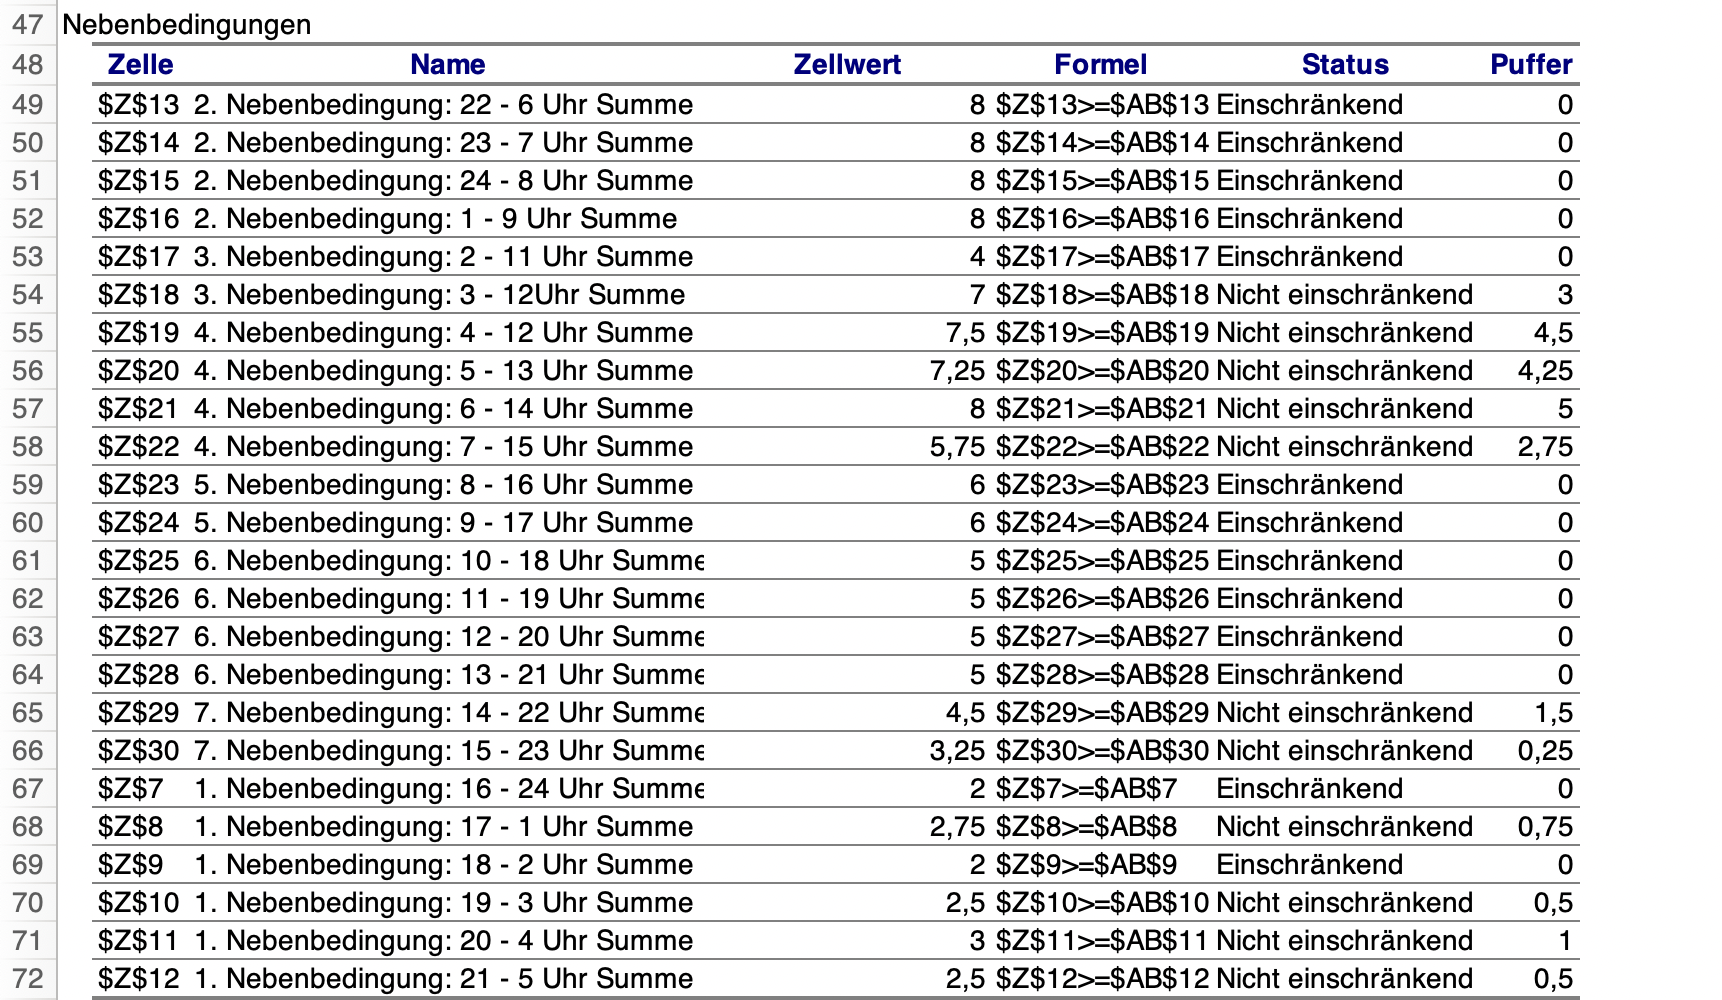
\includegraphics[width=17cm,left]{images/Antwortbericht13.png}\\~\\~\\~\\~\\~\\~\\\\\\
Sensitivitätsbericht 1:\\
\includegraphics[width=17cm,left]{images/Sensitivität11.png}
\includegraphics[width=17cm,left]{images/Sensitivität12.png}
\\\\\\\\\\\\\\\\\\
Grenzwertbericht 1:\\
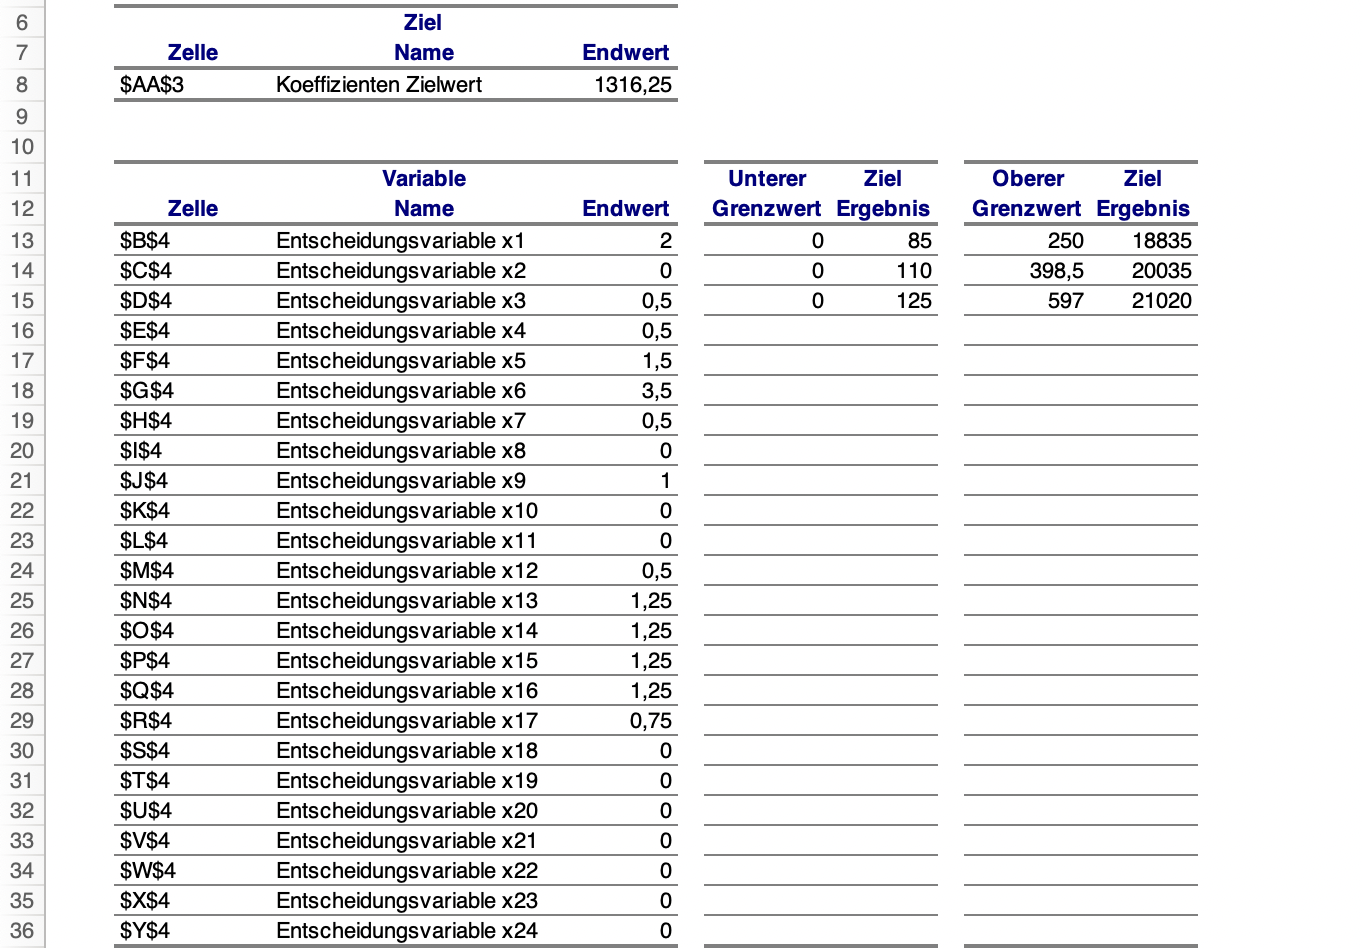
\includegraphics[width=17cm,left]{images/Grenzwert11.png}\\
%ja hier müssen so viele Umbrüche sein, da die Tabelle sonst zwischen 2 Seiten ist und nicht angezeigt wird
\\\\\\\\\\\\\\\\\\\\\\\\\\\\\\\\\\\\\\\\\\\\\\\\\\\\\\\\\\
Antwortbericht2:\\
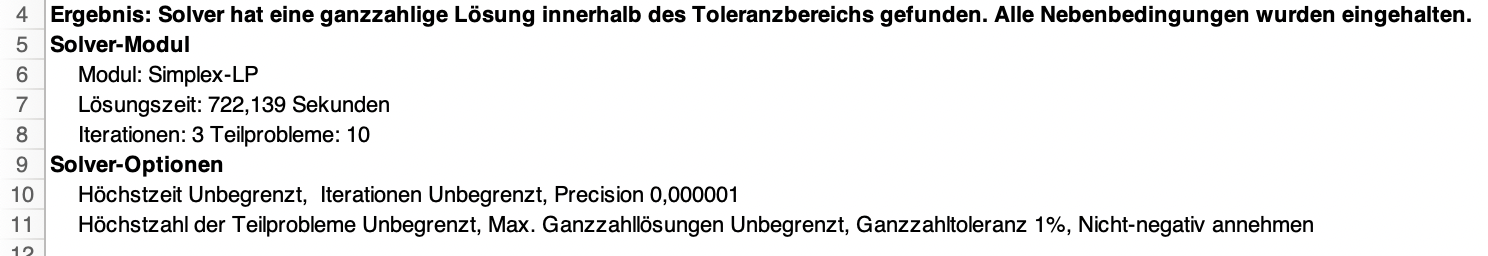
\includegraphics[width=17cm,left]{images/Antwortbericht21.png}
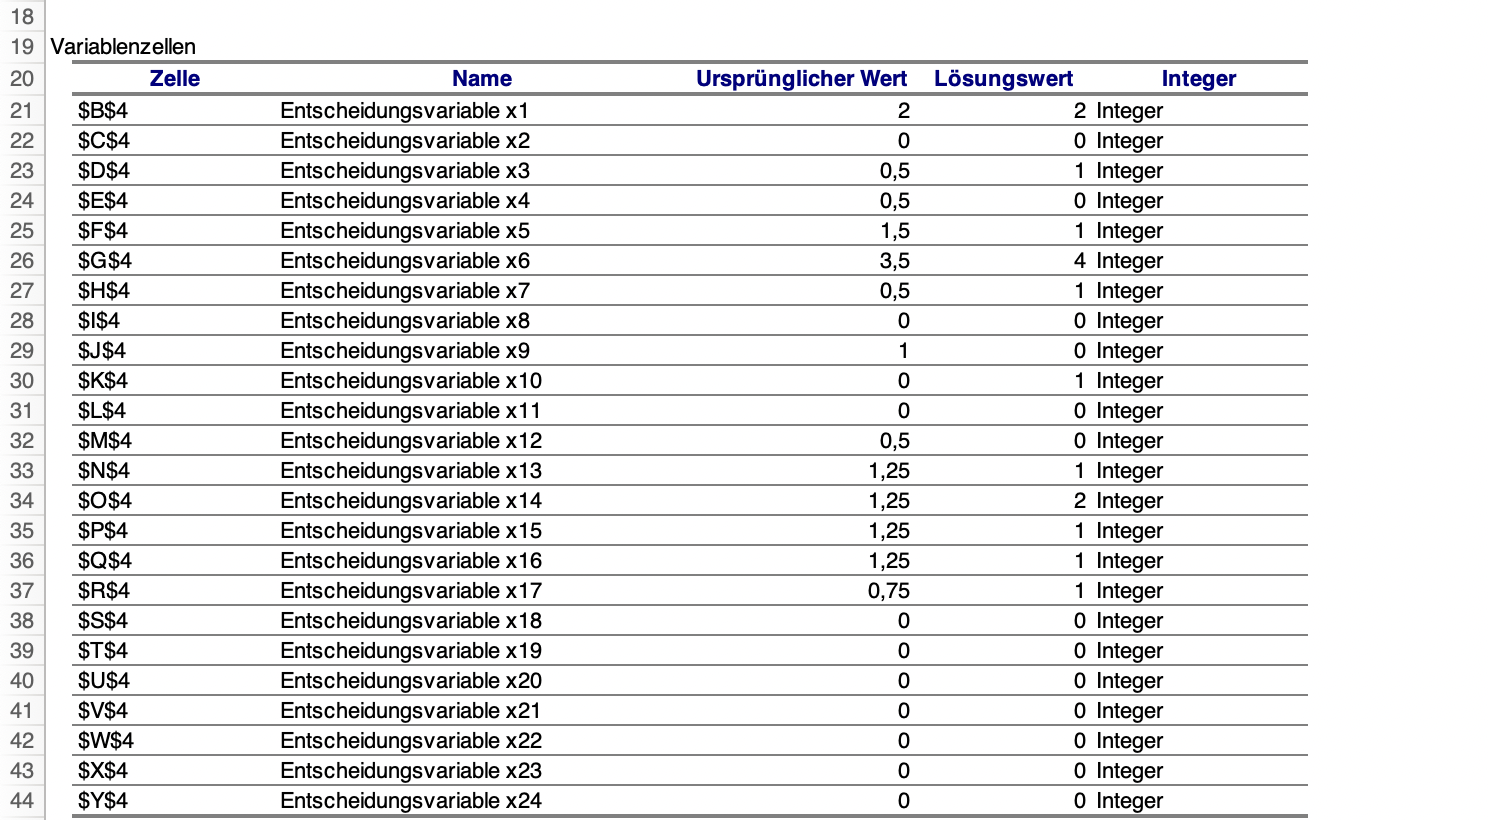
\includegraphics[width=17cm,left]{images/Antwortbericht22.png}
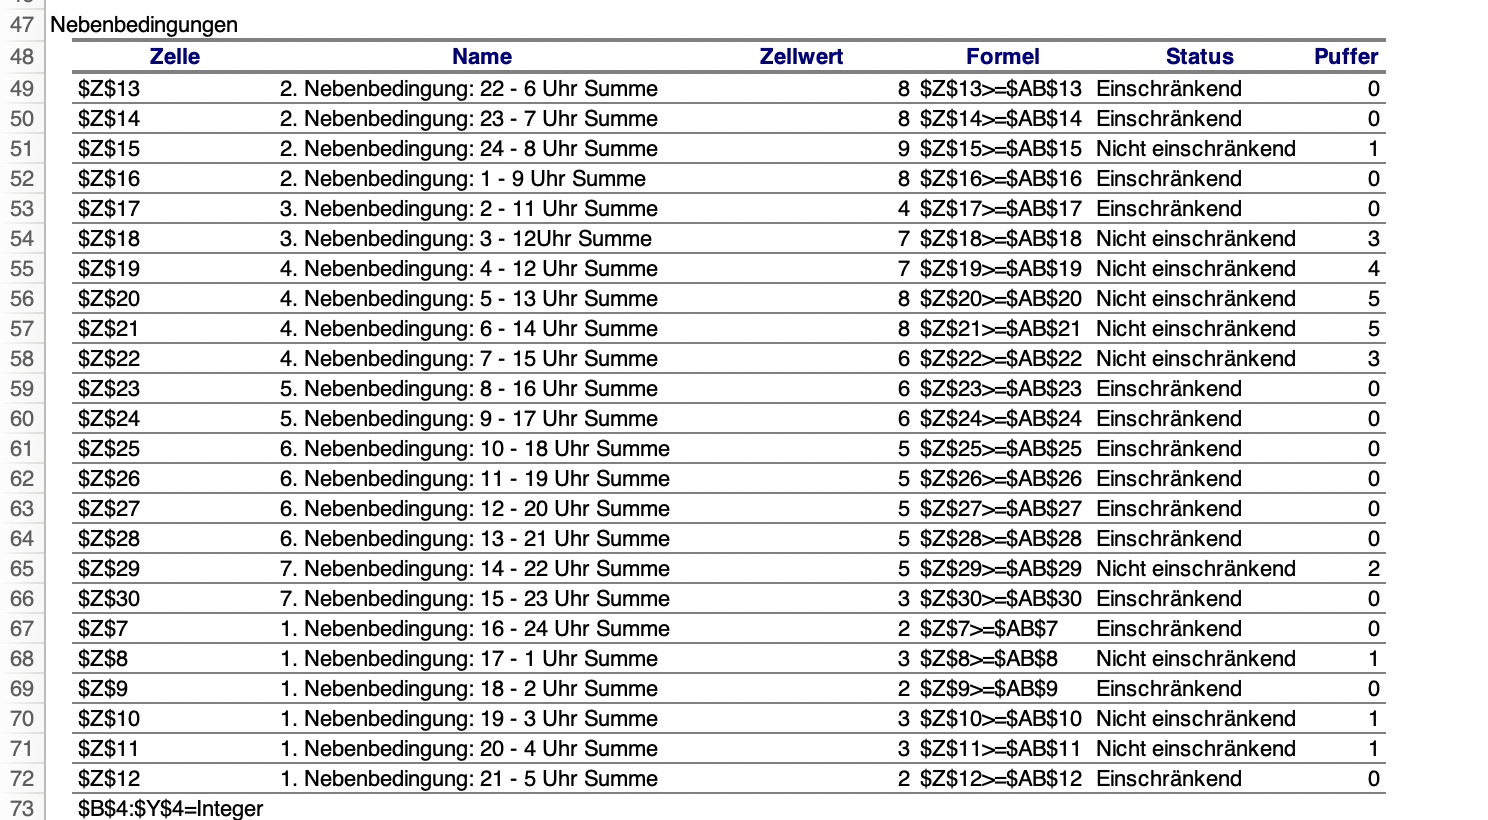
\includegraphics[width=17cm,left]{images/Antwortbericht23.png}



